\section{Trær}
\begin{figure}[H]
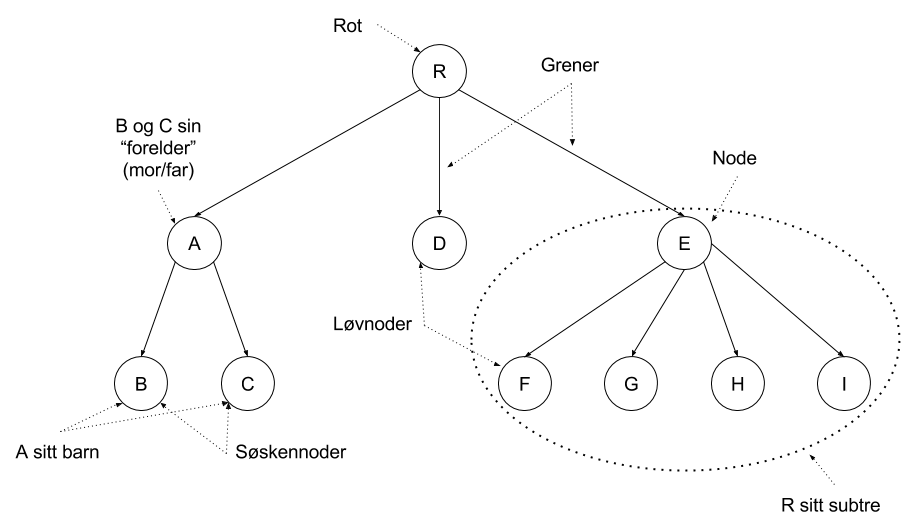
\includegraphics[scale=0.5]{images/traer}
\centering %centering the image
\caption{Tre}
\label{fig:trær}
\end{figure}

\begin{itemize}
    \item \textbf{Nivå for node} er antall grener som må passeres f.o.m. rot t.o.m. noden. Merk at rotnoden er på nivå 0.
    \item \textbf{Nodegrad} er antall barn (som er det samme som antall subtrær/undertrær) en node har.
    \item \textbf{Fritt tre} er at grenene ikke har retning, så alle nodene kan oppfattes som rotnode.
    \item \textbf{Rettet tre} vil si at grenene har retning, som i Figur \ref{fig:trær}.
    \item \textbf{Ordnet tre} vil si hvordan subtrærne/barna er ordnet i forhol til hverandre. Hvis det er viktig at A er til venstre, D i midten og E til høyre, er det et ordnet tre. Hvis rekkefølgen ikke har noe å si er det et uordnet tre.
    \item \textbf{Løvnode} er er node uten barn.
    \item \textbf{Indre node} er en node med barn.
    \item \textbf{Trehøyde} er maks antall grener som kan passeres f.o.m. rot t.o.m. løvnode.
    \item \textbf{$k$-grad-tre} vil si et tre der hver node kan ha maks $k$ barn. Posisjonen til barna er viktige.
    \item \textbf{Fullt $k$-grad-tre} er et $k$-grad-tre der alle indre noder har $k$ barn.
    \item \textbf{Komplett $k$-grad-tre} vil si et $k$-grad-tre der alle indre noder har $k$ barn, og enhver løvnode ligger på nivå $h$ eller $h - 1$, hvor $h$ er dybden (altså enten nederst i treet eller nest nederst). Antall noder på dybde $h$ er $k^h$. Trehøyden er $log_k n$ der $n$ er antall løvnoder.
\end{itemize}

\subsection{Implementasjon}
Hvordan vi implementerer en trestruktur avhenger av om vi har fast antall barn (f.eks. binære trær) eller variabelt antall barn (f.eks. B-trær).
\\\\
For hver av variantene har vi tatt med kjøretiden til to vanlige operasjoner:
\begin{itemize}
    \item finne forelder til en node
    \item finne barn nummer \textit{i} til en node
\end{itemize}

\noindent I generelle trær med fast antall barn har hver node er et objekt med en verdi, en peker til hver av barna og en peker til far.
\\\\
I generelle trær med variabelt antall barn er det to alternativer. Alternativ 1 er at hver node er et objekt med en verdi, en peker til sitt første barn (lengst til venstre), en peker til far og en til sin nærmeste bror til høyre for seg. I alternativ 2 utnytter vi at alle noder i et tre (untatt roten) har nøyatig én far. Vi lager en array. På plass nr \textit{i} står faren til node nummer \textit{i}, eller en peker til denne. Det blir da lett å finne faren, men for å finne barna til node \textit{i}, må vi søke gjennom arrayen etter tallet \textit{i}.

\begin{figure}[H]
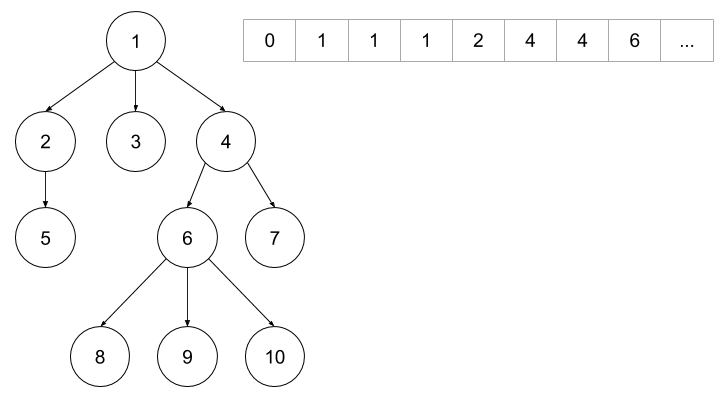
\includegraphics[scale=0.6]{images/fedrearray}
\centering %centering the image
\caption{Figuren viser et tre og den tilsvarende "fedrearrayen". Arrayen vil ha lke mange elementer som det er noder.}
\label{fig:fedrearray}
\end{figure}

\noindent Alternativ 3 er å lagre nodene i en array. HVert element i arrayen inneholder et objekt med verdien til noden og pekere til en lenket liste. Den lenkede listen inneholder pekere til barna.

\begin{figure}[H]
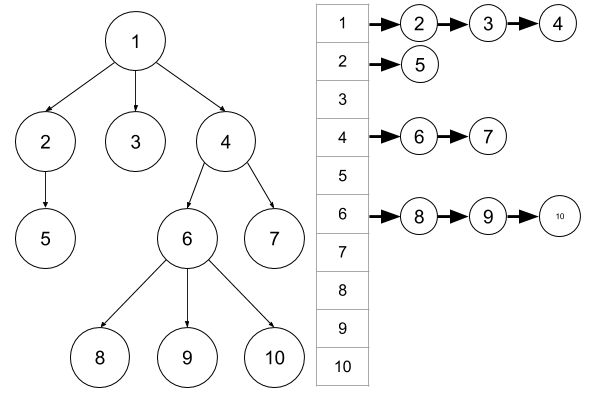
\includegraphics[scale=0.6]{images/alernativ3}
\centering %centering the image
\caption{Figuren viser alternativ 3.}
\label{fig:alternativ3}
\end{figure}

\subsection{Binære trær}
Binære trær er egentlig et 2-grad-tre, men dette navnet blir aldri brukt. Hver node har altså maks to barn og ordningen av høyre- og venstrebarn er viktig. Hver node er et objekt med en verdi, en peker til hver av barna og en peker til faren.

\begin{figure}[H]
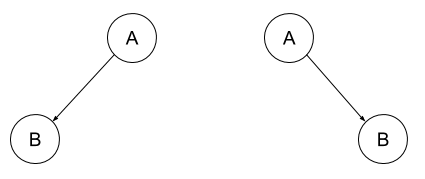
\includegraphics[scale=0.6]{images/binaeretraer}
\centering %centering the image
\caption{Disse to trærne er forskjellige!}
\label{fig:binaeretraer}
\end{figure}

\subsubsection{Binære søketrær}
Et binært søketre er bygget som et binært tre, men det er i tillegg organisert slik at verdien til venstre barn er mindre eller lik verdien til far mens verdien til høyre barn er større. Det betyr at for alle noder gjelder at alle verdiene til nodene i venstre subtre er lavere og alle i høyre er høyere enn verdien til noden selv. 

\begin{figure}[H]
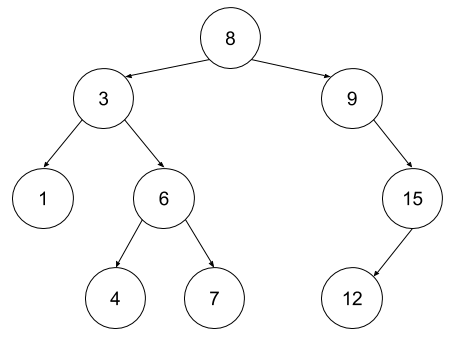
\includegraphics[scale=0.6]{images/binaeresoeketraer}
\centering %centering the image
\caption{Binært søketre}
\label{fig:binaeresoeketraer}
\end{figure}

\noindent Poenget er at med denne organiseringen er det vanligvis ganske kjapt å finne fram til ønsket node. Hvor lang tid det tar avhenger imidlertid av hvor heldig vi er med rekkefølgen nodene settes inn i. Hvor lang tid det tar å finne et element i verste tilfelle avhenger direkte av høyden til treet.  Forventet høyde for et tilfeldig binært søketre er $\theta(lg n)$. Det finnes søketrær med garantert høyde på $/theta(lg n)$.
\\\\
\textbf{Innsetting av node}\\
Innsetting av noder i et binært tre er enkelt. Det er bare å passe på å overholde kriteriene for et binærtre. Vi starter alltid ved roten. Dersom treet ikke har noen rot, dvs. treet ikke er påbegynt, settes vår node til å være rotnoden. Ellers sjekker vi for hver nye node vi kommer til om verdien til noden vi skal sette inn er større eller mindre enn verdien til denne noden. Dersom den er mindre, går vi til venstre, ellers går vi til høyre. Vår node kan settes inn på første tomme plass vi kommer til.

\begin{figure}[H]
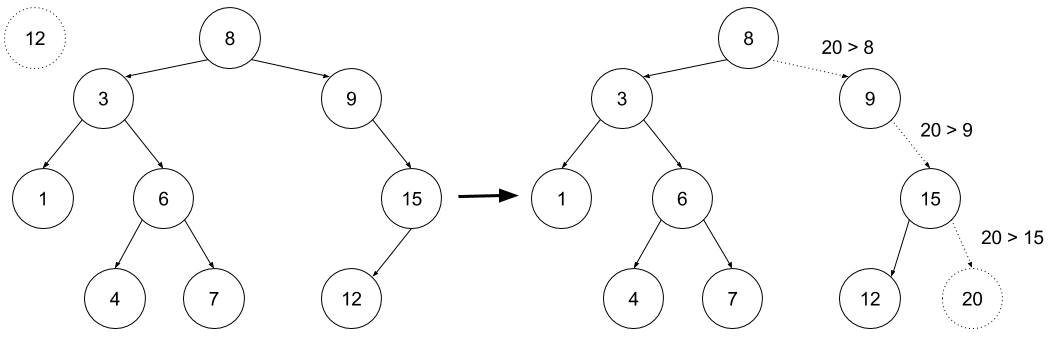
\includegraphics[scale=0.45]{images/innsettingnode}
\centering %centering the image
\caption{Sette inn node i binærtre}
\label{fig:innsettingnode}
\end{figure}

\noindent\textbf{Fjerning av node}\\
Vi har tre muligheter:
\begin{enumerate}
    \item \textbf{Noden vi skal fjerne har ingen barn.}\\ Vi kan da bare fjerne noden.
    \item \textbf{Noden vi skal fjerne har bare et barn.}\\ Vi kan da bare ta ut noden, og la barnet overta nodens far.
    \item \textbf{Noden vi skal fjerne har to barn.}\\ De to foregående tilfellene var enkle. Det er denne også, hvis man ser trikset. Spørsmålet vi må stille er: Hvilken annen node kan erstatte vår node, dvs. ta dens plass i treet? Det må være en med verdi større eller lik alle verdier i venstre subtre eller en med verdi mindre enn alle i høyre subtre. \newline \newline
    En løsning er å velge den noden med størst verdi i venstre subtre. Den finner du ved å gå til venstre barn og holde til høyre i hvert kryss videre nedover. Når du kommer til løvnoden har du funnet den du leter etter. \newline\newline
    En annen løsning er å velge den noden med minste verdi i høyre subtre. Helt tilsvarende går du da til høyre barn og holder til venstre i alle kryss helt til du når denne løvnoden.
    \newline\newline
    En av disse nodene kan klippes av og settes inn i stedet for den noden vi vil fjerne.
\end{enumerate}

\begin{figure}[H]
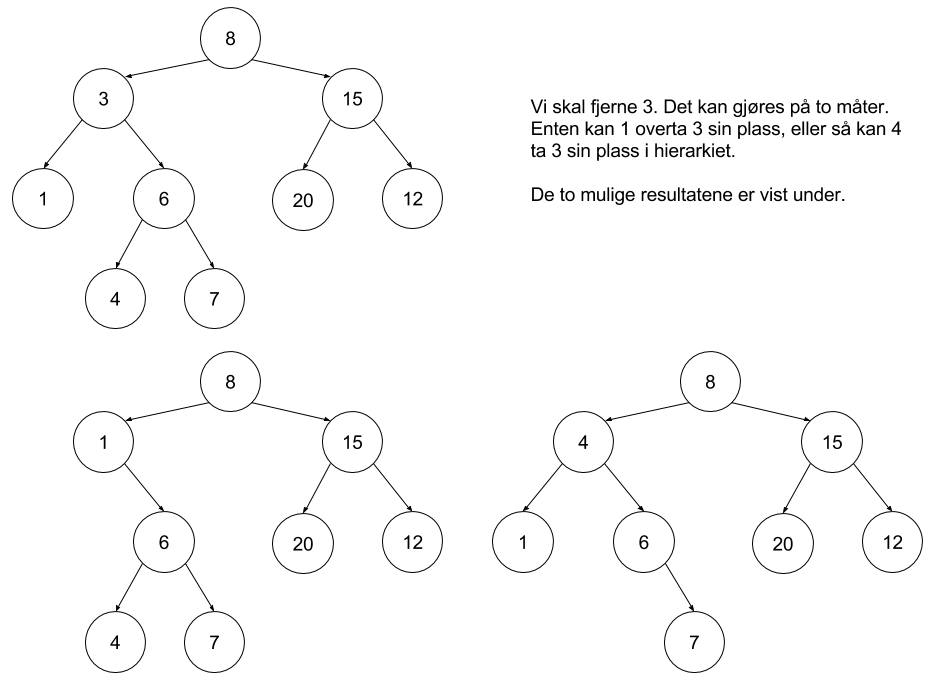
\includegraphics[scale=0.45]{images/fjernebarn}
\centering %centering the image
\caption{Fjerne barn}
\label{fig:fjernebarn}
\end{figure}

\subsection{Traversering}\\
Å traversere et tre eller en graf er et fint ord for å gå gjennom treet eller grafen. Her gir vi dere noen rekursive forklaringer på noen systematiske måter dette kan gjøres på.

\begin{itemize}
    \item \textbf{Prefiks:} Først utføres operasjonen på rotnoden, deretter prefikstraverseres venstre subtre (hvis det eksisterer) og til slutt prefikstraverseres høyre subtre (hvis det eksisterer). DFS. \textit{Kjører båt ved land, første man møter på.}
    \begin{figure}[H]
    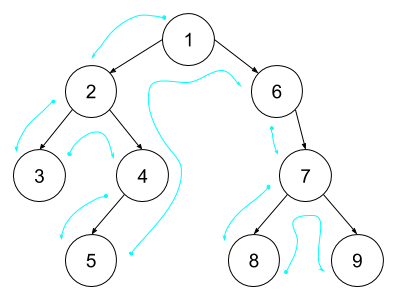
\includegraphics[scale=0.45]{images/prefiks}
    \centering %centering the image
    \caption{Prefikstraversering}
    \label{fig:prefiks}
    \end{figure}
    \item \textbf{Infiks:} Først infikstraverseres venstre subtre, deretter utføres operasjonen på rotnoden og til slutt infikstraverseres høyre subtre. DFS. 
    \begin{figure}[H]
    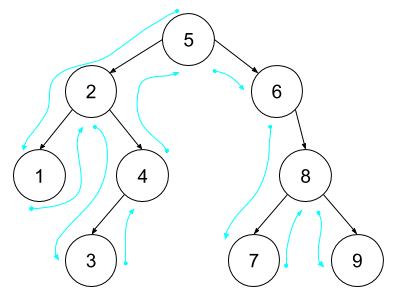
\includegraphics[scale=0.45]{images/infiks}
    \centering %centering the image
    \caption{Infikstraversering}
    \label{fig:infiks}
    \end{figure}
    \item \textbf{Postfiks:} Først postfikstraverseres venstre subtre, deretter høyre og til slutt utføres operasjonen på rotnoden. DFS. \textit{Siste på hver gren merkes.}
    \begin{figure}[H]
    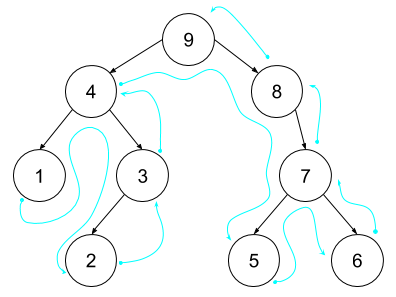
\includegraphics[scale=0.45]{images/postfiks}
    \centering %centering the image
    \caption{Postfikstraversering}
    \label{fig:postfiks}
    \end{figure}
    \item \textbf{Nivå:} Vi utfører først operasjonen på roten. Deretter tar vi for oss én og én rad på vei nediver, vanligvis fra venstre mot høyre. BFS. \textit{Merker fra venstre til høyre på hver rad.}
    \begin{figure}[H]
    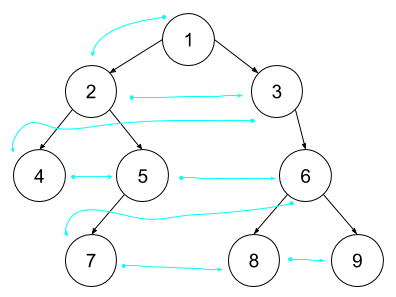
\includegraphics[scale=0.45]{images/nivaa}
    \centering %centering the image
    \caption{Nivåtraversering}
    \label{fig:nivå}
    \end{figure}
\end{itemize}

\begin{boxed}
\begin{itemize}
    \item \textbf{Preorder}: Her printer man ut nodens verdi før dens barn, venstre og deretter høyre. 
    \begin{itemize}
        \item Eksempel fra figuren under: 10, 6, 3, 2, 1, 4, 5, 8, 7, 9, 13, 11, 12, 18, 15, 14, 16, 17
    \end{itemize}
    \item \textbf{Inorder}: Her printer man venstre barn, noden, og deretter høyre barn (om ikke det er noe venstre barn, print noden før høyre barn)
    \begin{itemize}
        \item Eksempel fra figuren under: 1, 2, 3, 4, 5, 6, 7, 8, 9, 10, 11, 12, 13, 14, 15, 16, 17, 18
    \end{itemize}
    \item \textbf{Postorder}: Her printer man nodens verdi etter man har printet venstre og høyre barn
    \begin{itemize}
        \item Eksempel fra figuren under: 1, 2, 5, 4, 3, 7, 9, 8, 6, 12, 11, 14, 17, 16, 15, 18, 13, 10
    \end{itemize}
\end{itemize}

\begin{figure}[H]
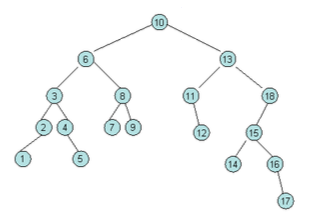
\includegraphics[scale=0.8]{images/tregraf}
\centering %centering the image
\caption{Tre}
\label{fig:tregraf}
\end{figure}
\end{boxed}

\subsection{Minimale spenntrær}
Som vi vet er et tre en forbundet graf uten sykler. Et \textbf{spenntre} er en subgraf av en graf \textit{G} som inneholder \textit{V - 1} kanter. Et \textbf{minimalt spenntre}, forkortet MST, av en vektet graf \textit{G} er et spenntre av \textit{G} som er slik at summen av kostnadene til kantene som inngår i treet, er minimal (det vil si at det ikke er mulig å lage andre spenntrær med mindre kantkostnader). Et MST er ikke nødvendigvis unikt – den kan altså finnes flere MST'er for samme graf.

\subsubsection{Prim}
Prinsippet med Prims algoritme er å alltid begynne med en tilfeldig node. I hvert steg ser man på alle kanter som forbinder en node som er med i treet man har bygget hittil med en node som ikke er med, og velger den kanten med minst kostnad. Dette gjøres ved å ha de ubrukte nodene i en prioritetskø, og markere hver node med den korteste kanten som forbinder den med en node i treet. Når alle nodene er med i treet, har du funnet et minimalt spenntre.
\\\\
Altså den mengden med kanter som minimerer summen av vekter samtidig som grafen er sammenhengende. Det minimale spenntreet reflekterer ikke nødvendigvis de faktisk korteste veiene fra en node til en annen.

\subsubsection{Kruskal}
Prinsippet med Kruskals algorimte er å sortere alle kantene etter kostnad, og se på kantene i stigende rekkefølge. Ta en kant (og nodene den går mellom) i spenntreet med mindre kanten ville ha laget en sykel. Fortsett til det ikke er flere kanter som kan legges til. Ideen er enkel, men for at algoritmen skal bli effektiv trenger man en avansert datastruktur som kalles \textit{disjoint set} for raskt å kunne finne ut om en kant vil danne en sykel eller ikke. Derfor anbefales Prim når man skal implementere en MST-algoritme selv.

\subsubsection{GENERIC-MST}
\subsubsection{MST-KRUSKAL}
\subsubsection{MST-PRIM}

\subsection{Spenntrær}
